% Generated fragments require trusted human review before compilation.
% This binder never requests shell escape or runs external tools.
\documentclass[11pt]{article}
% Trusted shared apparatus. Requires LuaLaTeX; never use shell escape.
\usepackage{fontspec}
\defaultfontfeatures{Ligatures=TeX}
\IfFontExistsTF{Noto Serif}{\setmainfont{Noto Serif}}{%
  \IfFontExistsTF{DejaVu Serif}{\setmainfont{DejaVu Serif}}{%
    \IfFontExistsTF{Times New Roman}{\setmainfont{Times New Roman}}{%
      \PackageError{gelfand-binder}{No configured Cyrillic serif font installed}{Install Noto Serif or DejaVu Serif, or select an installed Cyrillic font.}%
    }%
  }%
}
\IfFontExistsTF{Noto Sans}{\setsansfont{Noto Sans}}{%
  \IfFontExistsTF{DejaVu Sans}{\setsansfont{DejaVu Sans}}{\setsansfont{Arial}}%
}
\IfFontExistsTF{Noto Sans Mono}{\setmonofont{Noto Sans Mono}}{%
  \IfFontExistsTF{DejaVu Sans Mono}{\setmonofont{DejaVu Sans Mono}}{\setmonofont{Courier New}}%
}
\usepackage[a4paper,margin=22mm]{geometry}
\usepackage{amsmath,amssymb,amsthm,mathtools}
\usepackage{xcolor}
\usepackage{tikz}
\usepackage{tikz-cd}
\usetikzlibrary{arrows.meta,positioning,calc}
\usepackage{hyperref}
\hypersetup{unicode=true,colorlinks=true,linkcolor=blue,pdftitle={Gelfand transcription binder}}
\newtheorem{theorem}{Theorem}
\newtheorem{lemma}{Lemma}
\newtheorem{proposition}{Proposition}
\newtheorem{corollary}{Corollary}
\theoremstyle{definition}
\newtheorem{definition}{Definition}
\newtheorem{example}{Example}
\theoremstyle{remark}
\newtheorem{remark}{Remark}
\setlength{\parindent}{0pt}
\setlength{\parskip}{0.55em}
\setlength{\emergencystretch}{3em}
\newcommand{\SourcePage}[2]{%
  \clearpage\phantomsection\label{#1:source-page}%
  \addcontentsline{toc}{subsection}{#1}%
  {\small\sffamily\color{blue!60!black}Source scan frame: #1; visible page/leaf label: #2}\par\medskip%
}
\newcommand{\Unclear}[3]{%
  \begingroup\color{orange!70!black}%
  [Unresolved reading #1/#2: #3]\endgroup%
}
\newcommand{\Incomplete}[3]{%
  \par\begingroup\color{red!65!black}\textbf{Incomplete #1/#2:} #3\endgroup\par%
}
\newcommand{\SourceFigure}[3]{%
  \par\begingroup\color{blue!60!black}\textbf{\hyperref[#1:source-page]{Source figure #1/#2}:} #3%
  \par\textit{Consult the authoritative scan at this locator.}\endgroup\par%
}



% Reader layout only. Original diplomatic text is retained verbatim.
\setlength{\parskip}{0.35em}
\setlength{\emergencystretch}{4em}
\renewcommand{\SourcePage}[2]{%
  \par\addvspace{1em}\phantomsection\label{#1:source-page}%
  \addcontentsline{toc}{subsection}{#1}%
  {\footnotesize\sffamily\color{blue!55!black}#1%
    \def\givenlabel{#2}\def\nolabel{unlabelled}%
    \ifx\givenlabel\nolabel\else\quad[номер в источнике: #2]\fi
  }\par\nobreak\smallskip%
}
\renewcommand{\Unclear}[3]{%
  \begingroup\color{orange!65!black}%
  \ifmmode\text{[неясно: #3]}\else[неясно: #3]\fi\endgroup%
}
\renewcommand{\Incomplete}[3]{%
  \par\begingroup\color{red!60!black}\textbf{Неразобранный фрагмент:} #3%
  \endgroup\par%
}
\renewcommand{\SourceFigure}[3]{%
  \par\begingroup\color{blue!55!black}\textbf{Рисунок:} #3%
  \par{\small\textit{Исходный рисунок: \hyperref[#1:source-page]{#1}, #2.}}%
  \endgroup\par%
}
\hypersetup{pdftitle={Семинар И. М. Гельфанда. Дипломатическая транскрипция},pdfauthor={},pdfsubject={Русское рабочее издание с отмеченными сомнительными чтениями}}

\usepackage[normalem]{ulem}
\usepackage{newunicodechar}
\usepackage{adjustbox}
\newfontfamily\SourceSymbolFont{Segoe UI Symbol}
\newfontfamily\SourceCJKFont{MS Gothic}
\let\DiplomaticMathUnderline\underline
\renewcommand{\underline}[1]{\ifmmode\DiplomaticMathUnderline{#1}\else\uline{#1}\fi}
\newunicodechar{→}{\ifmmode\text{{\SourceSymbolFont\char"2192}}\else{\SourceSymbolFont\char"2192}\fi}
\newunicodechar{⇒}{\ifmmode\text{{\SourceSymbolFont\char"21D2}}\else{\SourceSymbolFont\char"21D2}\fi}
\newunicodechar{∀}{\ifmmode\text{{\SourceSymbolFont\char"2200}}\else{\SourceSymbolFont\char"2200}\fi}
\newunicodechar{∂}{\ifmmode\text{{\SourceSymbolFont\char"2202}}\else{\SourceSymbolFont\char"2202}\fi}
\newunicodechar{∈}{\ifmmode\text{{\SourceSymbolFont\char"2208}}\else{\SourceSymbolFont\char"2208}\fi}
\newunicodechar{∌}{\ifmmode\text{{\SourceSymbolFont\char"220C}}\else{\SourceSymbolFont\char"220C}\fi}
\newunicodechar{√}{\ifmmode\text{{\SourceSymbolFont\char"221A}}\else{\SourceSymbolFont\char"221A}\fi}
\newunicodechar{∞}{\ifmmode\text{{\SourceSymbolFont\char"221E}}\else{\SourceSymbolFont\char"221E}\fi}
\newunicodechar{∧}{\ifmmode\text{{\SourceSymbolFont\char"2227}}\else{\SourceSymbolFont\char"2227}\fi}
\newunicodechar{∩}{\ifmmode\text{{\SourceSymbolFont\char"2229}}\else{\SourceSymbolFont\char"2229}\fi}
\newunicodechar{∪}{\ifmmode\text{{\SourceSymbolFont\char"222A}}\else{\SourceSymbolFont\char"222A}\fi}
\newunicodechar{∫}{\ifmmode\text{{\SourceSymbolFont\char"222B}}\else{\SourceSymbolFont\char"222B}\fi}
\newunicodechar{∴}{\ifmmode\text{{\SourceSymbolFont\char"2234}}\else{\SourceSymbolFont\char"2234}\fi}
\newunicodechar{∼}{\ifmmode\text{{\SourceSymbolFont\char"223C}}\else{\SourceSymbolFont\char"223C}\fi}
\newunicodechar{≈}{\ifmmode\text{{\SourceSymbolFont\char"2248}}\else{\SourceSymbolFont\char"2248}\fi}
\newunicodechar{≠}{\ifmmode\text{{\SourceSymbolFont\char"2260}}\else{\SourceSymbolFont\char"2260}\fi}
\newunicodechar{≤}{\ifmmode\text{{\SourceSymbolFont\char"2264}}\else{\SourceSymbolFont\char"2264}\fi}
\newunicodechar{≥}{\ifmmode\text{{\SourceSymbolFont\char"2265}}\else{\SourceSymbolFont\char"2265}\fi}
\newunicodechar{⊕}{\ifmmode\text{{\SourceSymbolFont\char"2295}}\else{\SourceSymbolFont\char"2295}\fi}
\newunicodechar{⊗}{\ifmmode\text{{\SourceSymbolFont\char"2297}}\else{\SourceSymbolFont\char"2297}\fi}
\newunicodechar{①}{\ifmmode\text{{\SourceSymbolFont\char"2460}}\else{\SourceSymbolFont\char"2460}\fi}
\newunicodechar{②}{\ifmmode\text{{\SourceSymbolFont\char"2461}}\else{\SourceSymbolFont\char"2461}\fi}
\newunicodechar{③}{\ifmmode\text{{\SourceSymbolFont\char"2462}}\else{\SourceSymbolFont\char"2462}\fi}
\newunicodechar{④}{\ifmmode\text{{\SourceSymbolFont\char"2463}}\else{\SourceSymbolFont\char"2463}\fi}
\newunicodechar{Ⓗ}{\ifmmode\text{{\SourceSymbolFont\char"24BD}}\else{\SourceSymbolFont\char"24BD}\fi}
\newunicodechar{〃}{\ifmmode\text{{\SourceCJKFont\char"3003}}\else{\SourceCJKFont\char"3003}\fi}


% Reader revision 3. Annotation wording and candidates remain unchanged.
\setmainfont{NotoSerif-Regular.ttf}[Path=C:/Windows/Fonts/,ItalicFont=NotoSerif-Italic.ttf,BoldFont=NotoSerif-Bold.ttf,BoldItalicFont=NotoSerif-BoldItalic.ttf]
\usetikzlibrary{shapes.geometric,decorations.pathreplacing,decorations.markings,patterns,fit}
\newsavebox{\ReaderAnnotationBox}
\newcommand{\ReaderAnnotation}[1]{%
  \sbox{\ReaderAnnotationBox}{[неясно: #1]}%
  \ifdim\wd\ReaderAnnotationBox>.70\linewidth
    \parbox[t]{.70\linewidth}{\raggedright[неясно: #1]}%
  \else\usebox{\ReaderAnnotationBox}\fi%
}
\ExplSyntaxOn
\cs_new_protected:Npn \reader_unclear_candidate:n #1
 {
  \tl_set:Nx \l_tmpa_tl { \tl_to_str:n {#1} }
  % Text explicitly guarded inside a mathematical candidate remains math-safe.
  \regex_replace_all:nnN { \\(?:text|textrm|textnormal|textbf|operatorname)\s*\{[^{}]*\} } { } \l_tmpa_tl
  \regex_match:nVTF { [\x{0400}-\x{052F}] | \$ } \l_tmpa_tl
   { \ifmmode \text{\ReaderAnnotation{#1}} \else \ReaderAnnotation{#1} \fi }
   {
    \ifmmode
      [\text{неясно:~}#1]
    \else
      \regex_match:nVTF { [_^] | \\ } \l_tmpa_tl
       { \ensuremath{[\text{неясно:~}#1]} }
       { \ReaderAnnotation{#1} }
    \fi
   }
 }
\RenewDocumentCommand \Unclear { m m m }
 { \begingroup\color{orange!65!black}\reader_unclear_candidate:n{#3}\endgroup }
\ExplSyntaxOff
\newsavebox{\ReaderIncompleteBox}
\newcommand{\ReaderIncompleteNote}[1]{%
 \sbox{\ReaderIncompleteBox}{\textbf{Неразобранный фрагмент:} #1}%
 \ifdim\wd\ReaderIncompleteBox>.70\linewidth
  \parbox[t]{.70\linewidth}{\raggedright\textbf{Неразобранный фрагмент:} #1}%
 \else\usebox{\ReaderIncompleteBox}\fi%
}
\renewcommand{\Incomplete}[3]{%
 \ifmmode\text{\color{red!60!black}\ReaderIncompleteNote{#3}}%
 \else\leavevmode\begingroup\color{red!60!black}\ReaderIncompleteNote{#3}\endgroup\fi%
}
% Ragged right avoids stretching long untranslated abbreviations into margins.
\AtBeginDocument{\raggedright}
\newunicodechar{А}{\ifmmode\text{\char"410\relax}\else\char"410\relax\fi}
\newunicodechar{Б}{\ifmmode\text{\char"411\relax}\else\char"411\relax\fi}
\newunicodechar{В}{\ifmmode\text{\char"412\relax}\else\char"412\relax\fi}
\newunicodechar{Г}{\ifmmode\text{\char"413\relax}\else\char"413\relax\fi}
\newunicodechar{Д}{\ifmmode\text{\char"414\relax}\else\char"414\relax\fi}
\newunicodechar{Е}{\ifmmode\text{\char"415\relax}\else\char"415\relax\fi}
\newunicodechar{Ж}{\ifmmode\text{\char"416\relax}\else\char"416\relax\fi}
\newunicodechar{З}{\ifmmode\text{\char"417\relax}\else\char"417\relax\fi}
\newunicodechar{И}{\ifmmode\text{\char"418\relax}\else\char"418\relax\fi}
\newunicodechar{Й}{\ifmmode\text{\char"419\relax}\else\char"419\relax\fi}
\newunicodechar{К}{\ifmmode\text{\char"41A\relax}\else\char"41A\relax\fi}
\newunicodechar{Л}{\ifmmode\text{\char"41B\relax}\else\char"41B\relax\fi}
\newunicodechar{М}{\ifmmode\text{\char"41C\relax}\else\char"41C\relax\fi}
\newunicodechar{Н}{\ifmmode\text{\char"41D\relax}\else\char"41D\relax\fi}
\newunicodechar{О}{\ifmmode\text{\char"41E\relax}\else\char"41E\relax\fi}
\newunicodechar{П}{\ifmmode\text{\char"41F\relax}\else\char"41F\relax\fi}
\newunicodechar{Р}{\ifmmode\text{\char"420\relax}\else\char"420\relax\fi}
\newunicodechar{С}{\ifmmode\text{\char"421\relax}\else\char"421\relax\fi}
\newunicodechar{Т}{\ifmmode\text{\char"422\relax}\else\char"422\relax\fi}
\newunicodechar{У}{\ifmmode\text{\char"423\relax}\else\char"423\relax\fi}
\newunicodechar{Ф}{\ifmmode\text{\char"424\relax}\else\char"424\relax\fi}
\newunicodechar{Х}{\ifmmode\text{\char"425\relax}\else\char"425\relax\fi}
\newunicodechar{Ц}{\ifmmode\text{\char"426\relax}\else\char"426\relax\fi}
\newunicodechar{Ч}{\ifmmode\text{\char"427\relax}\else\char"427\relax\fi}
\newunicodechar{Ш}{\ifmmode\text{\char"428\relax}\else\char"428\relax\fi}
\newunicodechar{Щ}{\ifmmode\text{\char"429\relax}\else\char"429\relax\fi}
\newunicodechar{Ъ}{\ifmmode\text{\char"42A\relax}\else\char"42A\relax\fi}
\newunicodechar{Ы}{\ifmmode\text{\char"42B\relax}\else\char"42B\relax\fi}
\newunicodechar{Ь}{\ifmmode\text{\char"42C\relax}\else\char"42C\relax\fi}
\newunicodechar{Э}{\ifmmode\text{\char"42D\relax}\else\char"42D\relax\fi}
\newunicodechar{Ю}{\ifmmode\text{\char"42E\relax}\else\char"42E\relax\fi}
\newunicodechar{Я}{\ifmmode\text{\char"42F\relax}\else\char"42F\relax\fi}
\newunicodechar{а}{\ifmmode\text{\char"430\relax}\else\char"430\relax\fi}
\newunicodechar{б}{\ifmmode\text{\char"431\relax}\else\char"431\relax\fi}
\newunicodechar{в}{\ifmmode\text{\char"432\relax}\else\char"432\relax\fi}
\newunicodechar{г}{\ifmmode\text{\char"433\relax}\else\char"433\relax\fi}
\newunicodechar{д}{\ifmmode\text{\char"434\relax}\else\char"434\relax\fi}
\newunicodechar{е}{\ifmmode\text{\char"435\relax}\else\char"435\relax\fi}
\newunicodechar{ж}{\ifmmode\text{\char"436\relax}\else\char"436\relax\fi}
\newunicodechar{з}{\ifmmode\text{\char"437\relax}\else\char"437\relax\fi}
\newunicodechar{и}{\ifmmode\text{\char"438\relax}\else\char"438\relax\fi}
\newunicodechar{й}{\ifmmode\text{\char"439\relax}\else\char"439\relax\fi}
\newunicodechar{к}{\ifmmode\text{\char"43A\relax}\else\char"43A\relax\fi}
\newunicodechar{л}{\ifmmode\text{\char"43B\relax}\else\char"43B\relax\fi}
\newunicodechar{м}{\ifmmode\text{\char"43C\relax}\else\char"43C\relax\fi}
\newunicodechar{н}{\ifmmode\text{\char"43D\relax}\else\char"43D\relax\fi}
\newunicodechar{о}{\ifmmode\text{\char"43E\relax}\else\char"43E\relax\fi}
\newunicodechar{п}{\ifmmode\text{\char"43F\relax}\else\char"43F\relax\fi}
\newunicodechar{р}{\ifmmode\text{\char"440\relax}\else\char"440\relax\fi}
\newunicodechar{с}{\ifmmode\text{\char"441\relax}\else\char"441\relax\fi}
\newunicodechar{т}{\ifmmode\text{\char"442\relax}\else\char"442\relax\fi}
\newunicodechar{у}{\ifmmode\text{\char"443\relax}\else\char"443\relax\fi}
\newunicodechar{ф}{\ifmmode\text{\char"444\relax}\else\char"444\relax\fi}
\newunicodechar{х}{\ifmmode\text{\char"445\relax}\else\char"445\relax\fi}
\newunicodechar{ц}{\ifmmode\text{\char"446\relax}\else\char"446\relax\fi}
\newunicodechar{ч}{\ifmmode\text{\char"447\relax}\else\char"447\relax\fi}
\newunicodechar{ш}{\ifmmode\text{\char"448\relax}\else\char"448\relax\fi}
\newunicodechar{щ}{\ifmmode\text{\char"449\relax}\else\char"449\relax\fi}
\newunicodechar{ъ}{\ifmmode\text{\char"44A\relax}\else\char"44A\relax\fi}
\newunicodechar{ы}{\ifmmode\text{\char"44B\relax}\else\char"44B\relax\fi}
\newunicodechar{ь}{\ifmmode\text{\char"44C\relax}\else\char"44C\relax\fi}
\newunicodechar{э}{\ifmmode\text{\char"44D\relax}\else\char"44D\relax\fi}
\newunicodechar{ю}{\ifmmode\text{\char"44E\relax}\else\char"44E\relax\fi}
\newunicodechar{я}{\ifmmode\text{\char"44F\relax}\else\char"44F\relax\fi}
\newunicodechar{Ё}{\ifmmode\text{\char"401\relax}\else\char"401\relax\fi}
\newunicodechar{ё}{\ifmmode\text{\char"451\relax}\else\char"451\relax\fi}

\newunicodechar{æ}{\ifmmode\text{\char"E6\relax}\else\char"E6\relax\fi}
\newunicodechar{−}{\ifmmode\mathbin{\text{\SourceSymbolFont\char"2212\relax}}\else{\SourceSymbolFont\char"2212\relax}\fi}


% Reader-only pairing support; accepted raw bodies remain unchanged.
\RequirePackage{graphicx}
\RequirePackage{adjustbox}
\newcommand{\ReaderOriginalPanel}[2]{%
  \begin{minipage}[t]{.48\linewidth}\vspace{0pt}\centering
    \includegraphics[width=\linewidth,keepaspectratio]{#1}\par\smallskip
    {\scriptsize Оригинал рукописного рисунка: #2}\par
  \end{minipage}%
}
\newcommand{\ReaderDiagramPair}[3]{%
  \par\noindent\begingroup
  \ReaderOriginalPanel{#1}{#2}\hfill
  \begin{minipage}[t]{.48\linewidth}\vspace{0pt}\centering
    {\scriptsize Типографское воссоздание}\par\smallskip
    \begin{adjustbox}{max width=\linewidth}#3\end{adjustbox}\par
  \end{minipage}%
  \endgroup\par\smallskip
}
\newcommand{\ReaderDescriptionPair}[3]{%
  \par\noindent\begingroup
  \ReaderOriginalPanel{#1}{#2}\hfill
  \begin{minipage}[t]{.48\linewidth}\vspace{0pt}\raggedright
    {\scriptsize Типографское описание}\par\smallskip
    #3\par
  \end{minipage}%
  \endgroup\par\smallskip
}


\begin{document}
\begin{center}
{\Large Семинар И. М. Гельфанда}\par\medskip
{\LARGE Дипломатическая транскрипция}\par\bigskip
{\large Рабочее русское издание}\par\medskip
{\large Том 26 из 34. Архивная глава 026}\par\bigskip
Кадры GELFAND-P001199 -- GELFAND-P001218\par
\end{center}
\medskip
Сокращения, отменённые записи и сомнительные чтения сохранены.
Неразобранные фрагменты отмечены в тексте. Математические утверждения
источника переданы без молчаливых исправлений.

В текущем комплекте приняты 165 из 165 возвратов; учтены 1527 из 1527 кадров. Кадров без принятого возврата: 0.
Статусы кадров в отчётах о полноте: транскрибированы 1168, неразборчивы 357, частично прочитаны 1, недоступны 1.
Нерешённых записей журнала чтений: 6820.
Статус «неразборчивый» может отмечать локальную утрату зачёркнутой записи;
он не означает отсутствия всего кадра.
Сверка с рукописью продолжается. Рабочие журналы чтений и происхождения
данных сохранены отдельно.

Ограничения исходного комплекта: повреждённый исходный скан GELFAND-P000722; каталожные записи 603, 694 без сканов; в архивной главе 029 не перечислена часть 25.

Границы кадров показаны небольшими синими указателями; печатный текст
продолжается без обязательного разрыва страницы после каждого кадра.
\bigskip\hrule\bigskip
\SourcePage{GELFAND-P001199}{unlabelled}
\underline{9/IX-85 г.} \qquad \underline{\underline{Сем. Гельфанда.}}

\underline{\underline{Капранов Миша.}}

\underline{Функции Бейкера и их применения к уравнениям Янга-Миллса.}

Функция Бейкера произв. мн-зия
— простейшие ф-и с существ. особенностями.
\begin{equation*}
\varphi=e^{q(z)}\varphi_0,\qquad \varphi_0\text{ — голом.} \tag{1}
\end{equation*}
\begin{equation*}
q\in H^0(\mathcal O(D)/\mathcal O)
\overset{\delta}{\longrightarrow}H^1(\mathcal O)
\longrightarrow H^1(\mathcal O^*) \tag{2}
\end{equation*}
[В формуле (2) $H^0$ вписано над строкой перед первой скобкой.]

\begin{center}— $\cdot$ —\end{center}
\underline{Теперь что-то по мотивам Виттена,}

В $\mathbb C^{10|16}$ есть сем-во прямых размерности $1|8$.

В $\mathbb C^{10}$ есть скал. произведение
\begin{equation*}
\begin{gathered}
\langle\quad\rangle\quad\text{(симметрич.)}\\
\Downarrow\\
\text{0-е прямые отн. него}
\end{gathered}
\end{equation*}
[Справа, за двойной вертикальной чертой:]
($1|8$-расслоение 0-прямых)

[На левом поле:] \underline{А. Гончаров.}

$SO(10)$ действ. в $(\mathbb C^{10},\langle\, ,\,\rangle)$

$V_0\oplus V_1$,\quad $V_1$ — спинорное предст. группы
\Unclear{GELFAND-P001199}{spinor-group}{$SO(10)$}

$\dim V_1=16$

Подпр-ва разм. $(1,8)$: $L_0+L_1$

$L_0$ — 0-я прямая в $\mathbb C^{10}$ $\Longrightarrow$
подгруппа $SO(8)\subset SO(10)$

[Под правой частью:]
(в стабилизаторе прямой $L_0$)

(его полупростая часть — $SO(8)$)

Это группа вращ., сохр. $L_0$ и (содерж. его) ортог. дополнение

$\Longrightarrow$ получ. вращ. факторпр-ва.

Теперь спинорное предст. в
$SO(10)$ огранич. на $SO(8)$; получ. 2 инв. подпр. (8-мерных)

\SourcePage{GELFAND-P001200}{59}
$\Longrightarrow$ 2 сем-ва подпр-в.

[Зачёркнуто: \Unclear{GELFAND-P001200}{top-cancellation}{неразборчивые буквы}.]
Рассм. усл. интегрируемости нек-рой связности вдоль
[вписано над строкой: этих] подпр-в. Это
линейное условие на кривизну, совпад. с теми ур-ями, к-рые
были раньше написаны по другому поводу.

\begin{center}— $\cdot$ —\end{center}
\underline{Спинорное предст.}

\begin{equation*}
e_1,\ldots,e_{10}:\qquad e_i e_k+e_k e_i=2\delta_{ik}I
\end{equation*}
и порожд. ими кольцо

[Справа, за двойной вертикальной чертой:]
\begin{equation*}
\Unclear{GELFAND-P001200}{clifford-normalization}{x\cdot y+y\cdot x=(x,y)I}
\end{equation*}
Разм. кольца: $e_1,\ldots,e_{10};\quad e_i e_k,\quad e_i e_j e_k$
\qquad $(e_i^2=I)$

Всего $\dim=2^{10}$; оно простое (— изоморфно кольцу матриц)

[Под словом «матриц»:] $2^5\times2^5$

Получ. предст. разм. 32.

$A\in SO(10)$ не меняет ф-л $\Longrightarrow$ автом. кольца матриц,
он внутренний $\Longrightarrow$

$\Longrightarrow$ возникает представление.

\begin{center}— $\cdot$ —\end{center}
\underline{Кривизна на подпр-вах $=0$ $\Longleftrightarrow$
обобщ. автодуальное ур-е Янга-Миллса.}

Обычный Я.-М.: размерности 4 и 2.

\begin{center}— $\cdot$ —\end{center}
\SourceFigure{GELFAND-P001200}{projective-quadric-diagram}{Слева написано
$\mathbb{CP}^{12}$, причём последний знак показателя обведён повторно;
справа — $(\mathbb C^{12}\setminus0)/\mathbb C^*$.
Между ними стрелка влево, пересечённая длинной косой чертой.
Под левым обозначением стоят повёрнутый вертикально знак включения,
$Q_{10}$ и подпись «квадрика». Неясны окончательный показатель слева
и назначение косой черты на стрелке.}

[Справа от $Q_{10}$:]
есть какие-то направления
\Unclear{GELFAND-P001200}{super-direction-word}{суперн-ые}

\begin{center}— $\cdot$ —\end{center}
\underline{Преобр. Радона-Пенроуза.}

$\mathbb{CP}^3$; прямые в $\mathbb{CP}^3$ образуют $G(2,4)$
(2-мерн. подпр. в $\mathbb C^4$)

\begin{center}
\begin{adjustbox}{max width=\linewidth}
\begin{tikzcd}[column sep=large,row sep=large]
\mathbb C^4\setminus0 \arrow[d] &
(E,\nabla) \arrow[d] & \text{— рассл. со связностью} & F\text{ — кривизна}\\
\mathbb{CP}^3 & U\subset G(2,4) & &
\end{tikzcd}
\end{adjustbox}
\end{center}
[Под $U$ подписано: обл.]

$\alpha$-плоскости в $T_xU$: там имеется квадр. конус,
зад. скал. произвед.

В нём [над строкой вписано: 2] сем-ва 2-мерных
[зачёркнуто: \Unclear{GELFAND-P001200}{cone-cancellation}{неразборчивые буквы}]
подпр-в; выб. одно из них

$F|_{\Pi_\alpha}=0$ $\Longleftrightarrow$ рассл. наз. \underline{автодуальным.}

$G(2,4)$ имеет ранг 2 (1-е после сфер.); для совмещ. пары точек надо
задать 2 числа (а не одно как на сфере).

Кривизна $=0$ $\Longrightarrow$ автодуальное ур-е Я.-М.

$\rightsquigarrow$ другое рассл. над $\mathbb{CP}^3$;
$\alpha$-пов. — интегр. подмн-гие; расслоение
тривиализу. $\Longrightarrow$ дост. учесть слой над 1 точкой

[Справа, за двойной вертикальной чертой:]
Уже рассл. без связности на др. мн-зии.

\SourcePage{GELFAND-P001201}{unlabelled}
\underline{В.И. Арнольд.} \underline{О} \textit{[надстрочная вставка: (нек-рых)]} \underline{спец. ф-ях, возник. в теории бифуркаций.}

$H$ — многочлен

$H(x,y)=c$ — сем-во алг. кривых (вещ.)

$\omega=P\,dx+Q\,dy$ — форма ($P,Q$ — многочлены)
\begin{equation*}
\oint_{H=c}\omega=I(c)
\end{equation*}
Сколько нулей у интеграла $I(c)$?

В одном спец. случае реш. до конца.

\underline{Теорема} (\Unclear{GELFAND-P001201}{theorem-name}{Герман Петров-Танькин})

5-курсник, \Unclear{GELFAND-P001201}{student-note}{выгн.} из ун-та
\begin{equation*}
H=\frac{y^2}{2}+\underset{\text{многочлен}}{P_3(x)}
\end{equation*}
$c$ мен. в пределах инт., где \Unclear{GELFAND-P001201}{oval-word}{овалы}

$\operatorname{deg}P\le n,\quad\operatorname{deg}Q\le n.$

\SourceFigure{GELFAND-P001201}{phase-figure}{Справа две расположенные одна над другой кривые. Наверху кривая с максимумом слева и минимумом справа, две горизонтальные отметки справа и стрелка с подписью $c$, направленная влево к возрастающей ветви. Под ней горизонтальная линия пересекает большой замкнутый контур с остриём слева; внутри два меньших овальных контура. Видны вертикальные штрихи между рисунками и продолжение кривой справа вверх. Точные соединения штрихов не установлены.}

$\dim\{I\}=n$ (счёт при пом. \Unclear{GELFAND-P001201}{newton-abbreviation}{многогр.} Ньютона)

(интегралы — ф-и от $c$; они обр. лин. пр-во; т.к. $\omega$ можно склад.)

\tikz{\node[draw,circle] {!};} \underline{Утв.:} \underline{число нулей} $\overset{\text{любой рассм. ф-и}}{<n}$ (если она $\ne0$)

ф-и удовл. ур-ю Пикар--Фукса (связн. Гаусса--Манина)

\underline{Комментарий:} \Unclear{GELFAND-P001201}{linear-combination-claim}{$\forall f_1,\ldots,f_N$ комбин. $c_1f_1+\cdots+c_Nf_N$ имеет $N-1$ нуль (если лин. независ.)}

Если число нулей $<\dim$, то сист. наз. \underline{чебышевской}

(\underline{неосцилляция})

\underline{Вопрос:} связь с осцилл. теоремами?

\underline{Счёт $\dim$:} $\int=0$ если а) полный диффер.

б) умн. чего-то на $H-c$.

\underline{Использование многогранника Ньютона для выч. размерностей}

$f=x^3+y^4;\qquad \mathbb{C}[[x,y]]/(\frac{\partial f}{\partial x},\frac{\partial f}{\partial y})$

\begin{adjustbox}{max width=\linewidth}
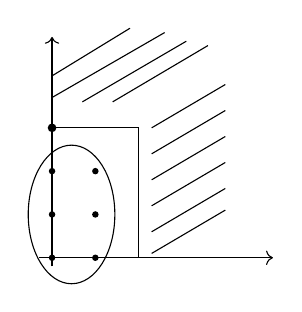
\begin{tikzpicture}[x=0.55cm,y=0.55cm]
\draw[->] (-0.3,0) -- (5.1,0);
\draw[->] (0,-0.2) -- (0,5.1);
\draw (0,3) -- (2,3) -- (2,0);
\draw (0,4.2) -- (1.8,5.3);
\draw (0,3.7) -- (2.6,5.2);
\draw (0.7,3.6) -- (3.1,5.0);
\draw (1.4,3.6) -- (3.6,4.9);
\draw (2.3,3.0) -- (4.0,4.0);
\draw (2.3,2.4) -- (4.0,3.4);
\draw (2.3,1.8) -- (4.0,2.8);
\draw (2.3,1.2) -- (4.0,2.2);
\draw (2.3,0.6) -- (4.0,1.6);
\draw (2.3,0.1) -- (4.0,1.1);
\fill (0,0) circle (0.075);
\fill (1,0) circle (0.075);
\fill (0,1) circle (0.075);
\fill (1,1) circle (0.075);
\fill (0,2) circle (0.075);
\fill (1,2) circle (0.075);
\fill (0,3) circle (0.10);
\draw (0.45,1) ellipse (1.0 and 1.6);
\end{tikzpicture}
\end{adjustbox}

базис факторпр-ва. $\dim=6$

$x^2y+y^4$

\SourceFigure{GELFAND-P001201}{newton-right-figure}{В нижнем правом рисунке вертикальная и горизонтальная оси без подписей. На вертикальной оси над короткой отметкой расположен квадрат; правее квадрата на той же высоте кружок с внутренними штрихами, ниже него треугольник. На горизонтальной оси две короткие отметки, затем квадрат и кружок с внутренними штрихами. Внутренние знаки квадрата и кружков не установлены. Под рисунком стрелка $\Rightarrow$ и подчёркнутое слово «базис».}

\SourcePage{GELFAND-P001202}{60}
\underline{А. Зелевинский.} О «самом красивом результате в обл. чистой мат.»

(Тройное тожд. Якоби)
\begin{equation*}
\sum_{r=-\infty}^{\infty}z^r q^{r^2}
=\prod_{k=1}^{\infty}(1-q^{2k})(1+q^{2k-1}z)(1+q^{2k-1}z^{-1})
\tag{1}
\end{equation*}
(тройное тожд. Якоби)
\begin{equation*}
\Vert
\end{equation*}
\begin{center}
\Unclear{GELFAND-P001202}{pochhammer-product}{$(1;q^2)_\infty(-zq^{-1};q^2)_\infty(-z^{-1}q^{-1};q^2)_\infty$}
\end{center}

Здесь
\begin{equation*}
(a;q)_\infty:=\prod_{n=0}^{\infty}(1-aq^n)
\end{equation*}
!! Выводится из \underline{тожд. Рамануджана.}

\underline{Комбинаторное док-во}

Первое произв. перенесём в лев. часть
\begin{equation*}
\left(\sum_{r=-\infty}^{\infty}z^r q^{r^2}\right)
\prod_{k=1}^{\infty}(1-q^{2k})^{-1}
=\prod_{k=1}^{\infty}(1+q^{2k-1}z)(1+q^{2k-1}z^{-1})
\tag{2}
\end{equation*}
\Unclear{GELFAND-P001202}{equation-two-cancellation}{[Зачёркнутый знак над $z^r$ в левой части (2).]}

Отличен от $0$ только коэфф. при $\underline{z^r q^{r^2+2n}}$

(и слева и справа)

$={}$ число разбиений числа $n$ на слаг. $=p(n)$

(слева)

(3) \underline{Справа:} подсчитаем
\begin{equation*}
\alpha_1>\alpha_2>\cdots>\alpha_s>0
\end{equation*}
неч.

\Unclear{GELFAND-P001202}{beta-inequalities}{$\beta_1>\beta_2>\cdots>\beta_t>0$}
\begin{equation*}
\sum\alpha_j+\sum\beta_i=r^2+2n,\qquad \underline{\underline{s-t=r}}
\end{equation*}
\textit{[От «неч.» два расходящихся штриха к строкам $\alpha$ и $\beta$; слева и справа от строк проведены вертикальные разделители.]}

\Unclear{GELFAND-P001202}{both-descriptions}{И то и другой}
(\Unclear{GELFAND-P001202}{leibenzon-name}{З.Л. Лейбензон}) — комбинат. описание мн-ва:
\begin{equation*}
00000\,1\,0000\,1\,00\,111111
\end{equation*}
беск. слова (\underline{сцепления})

\Unclear{GELFAND-P001202}{cancelled-left-word}{[Зачёркнуто: слева]}
снач. беск. число $0$; потом каша; потом \underline{палочки}

(беск. число)

Высота: $h(A)$ — число инверсий $\underbrace{1\,0}$ — как угодно далеко друг от друга

$\underline{h(A)=n}\quad\Rightarrow$ число элем. $p(n)$

— параметриз. наборами вида (3).

\underline{1-й способ}
\begin{equation*}
0000\,1\,0\,111\qquad\text{— выс. }1
\end{equation*}
$p(n)$ — возьмём лев. палочку, счит. за ней нули и т.д.

\underline{2-й способ}

Пробелы имеют \textit{[над «номер»: (естеств.)]} номер: (число $1$ слева) — (число $0$ справа)

\underline{Номер} мен. от $-\infty$ до $+\infty$ !! (всюду!)

\SourcePage{GELFAND-P001203}{unlabelled}
\underline{Замет. Арнольда:}

Изобразим:

$0$ — ход вправо

$1$ — ход вверх

\begin{adjustbox}{max width=\linewidth}
\begin{tikzpicture}[x=0.48cm,y=0.38cm]
\draw (-4,0) -- (0,0) -- (0,1) -- (2,1) -- (2,2) -- (3,2) -- (3,4) -- (4,4) -- (4,7);
\draw[line width=1.4pt] (3,4) -- (4,4);
\node at (-0.35,-0.38) {$0$};
\node at (-0.3,0.5) {$1$};
\node at (0.5,1.4) {$0$};
\node at (1.5,1.4) {$0$};
\node at (2.28,1.5) {$1$};
\node at (2.5,2.4) {$0$};
\node at (3.3,2.5) {$1$};
\node at (3.3,3.5) {$1$};
\node at (3.5,4.4) {$0$};
\node at (4.3,4.5) {$1$};
\node at (4.3,5.5) {$1$};
\node at (4.3,6.5) {$1$};
\end{tikzpicture}
\end{adjustbox}

диагр. Юнга

ф-я $\underline{x-y}$ \underline{нумерует} все

Рассм. пробел с номером $r$.

Сцепление характеризуем так:

расст. от пробела до палочек, \textit{[под словом с фигурным указателем: леж. слева]} $\Vert$ \underline{нечётные числа}.

— ″ — кружочков. \textit{[под словом с фигурным указателем: леж. справа]}
\begin{equation*}
\sum\alpha_j+\sum\beta_j=r^2+2n
\end{equation*}
из площади под кривой.

16/IX-85г. \underline{Сем. Гельфанда.}

\underline{Зелевинский} (и Бейлинсон) со слов \underline{M.-F. Vigneras} (Marie-France Vigneras)

\Unclear{GELFAND-P001203}{name-aside}{[Надстрочная помета в скобках: Ma'...ia.]}

1) о раб. «From \Unclear{GELFAND-P001203}{lifting-field-notation}{$\mathrm{GL}(2,\mathbb{Q}\sqrt d)$} to $\mathrm{GSp}(4,\mathbb{Q})$» (M.-F. Vigneras)

Стр. соотв. между представлениями.

(лифтинг)

При переходе к $p$-адич. полю

это позволяет проверить для $\mathrm{GSp}(4,F)$ какую-то гипотезу Ленглендса

о функториальности.

\textit{[Справа, с указателем к $\mathrm{GSp}$:]} симплект. подобия (сохр. симпл. форму с точн. до множителя)

\textit{[Под $F$:]} $p$-адич.

2) \underline{Rallis, Пятецкий--Шапиро и др.}
\begin{equation*}
L(s,\pi_1\times\pi_2\times\pi_3),\quad\text{где }\pi_j\text{ — предст. }\mathrm{GL}_2(F)
\end{equation*}
3) По рассказу \Unclear{GELFAND-P001203}{latin-surname}{Jacket} «Как использовать ф-лу следа?»

\Unclear{GELFAND-P001203}{result-abbreviation}{Пол.} важный результат — теор. Пэли--Винера,
\Unclear{GELFAND-P001203}{cancelled-theorem-phrase}{[Зачёркнутая фраза перед «док.».]}
док. Кажданом и Бернштейном.

\textit{[В овале, соединённом с заглавием о результате:]} о предст. над $F$

$G$ — редукт. $p$-адич. гр. (напр. $\mathrm{GL}_n$)

\Unclear{GELFAND-P001203}{hecke-superscript}{$H^{\bullet}(G)$} —
\Unclear{GELFAND-P001203}{algebra-insertion}{[надстрочная вставка с указателем после тире: (алг.)]} лок. пост. финитных ф-й на $G$.

лок. пост. заменяют $C^\infty$-ф-и

По $f$ строим:
\begin{equation*}
\pi\longrightarrow\operatorname{tr}\pi(f)
\end{equation*}
— функцию на $\operatorname{Irr}G$

Здесь
\begin{equation*}
\pi(f)=\int_G f(g)\pi(g)\,dg
\end{equation*}
\underline{Теорема} (Пэли--Винера и К.-Б.) даёт описание всех таких ф-й

Непр. предст. делятся на листы и сем-ва: по $\rho\in\operatorname{Irr}M$ строится

$M\subset G$
\begin{equation*}
\pi\in\mathrm{JH}\;\operatorname{Ind}_{P}^{G}\rho
\end{equation*}
(ряд Жорд.--Гельдера)

$\Vert$ каждое сем-во приобрет. структуру

$M$ — подгр. Леви параб. подгруппы в $G$

(полупр. часть)

характер непр. предст. $\Leftrightarrow$ \underline{алгебраичность} нек-рой ф-и

Идея в вещ. \textit{[под «вещ.» в обводке: и компл.?]} случае: \Unclear{GELFAND-P001203}{final-verb}{убыв.} на $\forall$ картановской подалгебре

\SourcePage{GELFAND-P001204}{61}
\underline{M.-F. Vigneras.} \quad (об этом же, но более \Unclear{GELFAND-P001204}{upper-aside-final}{точн.})

$G$ reductive $p$-adic group (напр., $GL_n$)
\begin{equation*}
\coprod_{(M,\rho)}\{\rho\chi\}^{W}=\operatorname{Irr}G \tag{1}
\end{equation*}
[Подписи с выносными линиями: к $M$ —
\Unclear{GELFAND-P001204}{upper-m-caption}{станд.}
ред. подгр.; к $\rho$ — неприв. куспидальное предст.;
к $\chi$ — неразветвл. характер; к $W$ — с точн. до действия гр. Вейля.]

$\{\rho\chi\}^{W}$ — конечномерное алг. мн-же (над $\mathbb C$).

по $f\in H(G)$ оп. ф-я на [вставлено: мн-ве (1)]
\begin{equation*}
\pi\longrightarrow\operatorname{trace}\operatorname{ind}_{M}^{G}\rho\chi(f)
\end{equation*}
Условия

а) алгебраична на $\forall$ таком мн-же

б) сосредот. на их конечном числе

\underline{\underline{Бейлинсон.}}

[Зачёркнуто:
\Unclear{GELFAND-P001204}{middle-beilinson-cancel}{неразборчиво}.]

Предст. $GSp(4,\mathbb Q)$ — ?
\begin{equation*}
W_{\mathbb Q_p}\subset\operatorname{Gal}(\overline{\mathbb Q}_p/\mathbb Q_p)
\end{equation*}
\begin{equation*}
\operatorname{Irr}GSp(4,\mathbb Q)\longrightarrow
\Unclear{GELFAND-P001204}{middle-wd-sign}{\text{неразборчивый знак}}
\quad\text{предст. гр. Вейля-Делиня}
\end{equation*}
[Подпись с выносной линией к правой части стрелки:]
прообр. $\forall$ точки конечен ($L$-пакет)
\begin{equation*}
GL(2,\mathbb Q(\sqrt d))\longrightarrow GO(4)
\end{equation*}
\begin{equation*}
\left\{x\in M(2,\mathbb Q(\sqrt d)):
\Unclear{GELFAND-P001204}{middle-hermitian-condition}{x=\bar x}\right\}
\qquad
x=\begin{pmatrix}a&b\\\bar b&d\end{pmatrix}
\end{equation*}
$\det$ — кан. квадр. форма \qquad (он рационален)
\begin{equation*}
x\longmapsto gx\bar g^{t}\qquad\text{сохр. это условие}
\end{equation*}
(аналог спинорного предст.)

Предст. Вейля: предст. $GO(4)\times GSp(4)$

оно реализуется в $\theta$-ф-ях

\underline{\underline{Б. Фейгин.}} \qquad \underline{О струнах}

[Зачёркнуто:
\Unclear{GELFAND-P001204}{lower-theory-cancel}{неразборчиво}.]
Теория струн — статистика поверхностей.

Квант. мех. изучает пр-во с лагранжианом; действие зав. от траектории.

Струны: вместо траектории — поверхность.

$\mathcal E$ — риманова пов., рассм. пр-во $\mathbb R^d$

Траект. — отобр.
\begin{equation*}
\underset{x_1,\ldots,x_d}{\{\mathcal E\longrightarrow\mathbb R^d\}}.
\end{equation*}
\underline{Идея:} все элем. част. опис. отображениями $\mathcal E$ в суперпр-во $\mathbb R^{10/m}$

Движ. окружности — поверхность
\begin{center}
\begin{adjustbox}{max width=\linewidth}
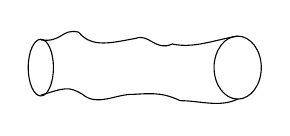
\begin{tikzpicture}[x=1cm,y=1cm]
\draw (0,0) ellipse (0.16 and 0.36);
\draw (2.5,0) ellipse (0.3 and 0.4);
\draw (0,0.35) .. controls (0.28,0.32) and (0.26,0.50) .. (0.48,0.45)
 .. controls (0.65,0.24) and (0.91,0.32) .. (1.2,0.37)
 .. controls (1.38,0.44) and (1.45,0.20) .. (1.67,0.30)
 .. controls (1.94,0.24) and (2.2,0.35) .. (2.5,0.4);
\draw (0,-0.35) .. controls (0.3,-0.26) and (0.35,-0.23) .. (0.53,-0.34)
 .. controls (0.72,-0.5) and (0.96,-0.33) .. (1.18,-0.34)
 .. controls (1.46,-0.32) and (1.58,-0.33) .. (1.77,-0.42)
 .. controls (2.02,-0.42) and (2.27,-0.51) .. (2.5,-0.4);
\end{tikzpicture}
\end{adjustbox}
\end{center}
Класс. аналог — рост кристалла.

\SourcePage{GELFAND-P001205}{unlabelled}
Лагранжиан:
\begin{equation*}
\mathcal L=\int
\Unclear{GELFAND-P001205}{upper-lagrangian-cancel}{\text{[зачёркнуто: неразборчиво]}}
(\det g_{ij})^{1/2}\,d\sigma\,d\tau
\qquad\text{(лагранжиан Намбу)} \tag{1}
\end{equation*}
(площадь в индуц. метрике)

Надо рассм. фейнмановский интеграл.
\begin{equation*}
X:\mathcal E\hookrightarrow\mathbb R^d
\end{equation*}
Другая запись (1):
\begin{equation*}
\mathcal L(X)=\int d\sigma\,d\tau
\left[\left(\frac{\partial X}{\partial\sigma}\right)^2
\left(\frac{\partial X}{\partial\tau}\right)^2
-\left(\frac{\partial X}{\partial\sigma}\cdot
\frac{\partial X}{\partial\tau}\right)^2\right]^{1/2} \tag{1'}
\end{equation*}
Фейнман. интеграл
\begin{equation*}
\int e^{\beta\mathcal L(X)}\,\mathcal D X \tag{2}
\end{equation*}
Есть 2 подхода: через интегр. и через обычные операторы (!) и теперь установлено соответствие.

\underline{Поляков:} другой контин. интеграл

$\widetilde X$ — [вставлено: пр-во] элементы к-рого — пары

1) $X:\mathcal E\longrightarrow\mathbb R^d$

2) $g_{ij}$ на $\mathcal E$ (рим. метрика на $\mathcal E$)

Лагранжиан Полякова:
\begin{equation*}
\Unclear{GELFAND-P001205}{lower-lagrangian-cancel}{\text{[зачёркнуто: неразборчиво]}}
\mathcal L=
\Unclear{GELFAND-P001205}{lower-lagrangian-coefficient}{\text{æ}}
\int(\det g_{ij})^{1/2}
+\int\frac{\partial X_i}{\partial\xi_\alpha}
\frac{\partial X_i}{\partial\xi_\beta}g^{\alpha\beta}
\overset{\text{[вставлено]}}{\sqrt g}\,d\xi_1\,d\xi_2 \tag{3}
\end{equation*}
[Вставлено: К нему] Применима техника вычисления

Способ работы: фиксируем $g_{ij}$ и вычисляем интеграл по $X$ — он квадратичный.
\begin{center}— $\cdot$ —\end{center}

\SourcePage{GELFAND-P001206}{62}
\underline{23.9.85 г.} \quad \underline{Сем. Гельфанда.}

\underline{И.М.Г.} \underline{Задача (для 9 кл.)}
Какой многогранник получается в сечении 4-мерного куба
3-мерной гиперплоскостью, проходящей через центр и перпендикулярной главной диагонали?

\underline{А. Бейлинсон.} О новой серии раб. Пятецкого-Шапиро и Раллиса.

функц. ур-я $L$-ф-и, связ. с автом. формами

$G$ — полупр. группа над $\mathbb Q$ (напр., гр. матриц $n\times n$)

$G/\mathbb Q$.
\Unclear{GELFAND-P001206}{upper-gq-cancel}{[неразборчивые зачёркнутые знаки]}

\underline{Задача:} описать представления адельной группы $G(A)$ в
\Unclear{GELFAND-P001206}{upper-l2-parentheses}{$L^2(G(A)/G(\mathbb Q)$}

Соотв. представл. наз. \underline{автоморфными}.
\begin{center}— $\cdot$ —\end{center}
\underline{И.М.Г.} $\forall$ нат. число запис. в виде
\begin{equation*}
a_0+a_1p+a_2p^2+\ldots+a_np^n
\end{equation*}
Всякое рац. число
\begin{equation*}
\Unclear{GELFAND-P001206}{middle-rational-expansion}{a_{-m}p^{-m}+a_1p^{-m+1}+\ldots+a_kp^k+}
\end{equation*}
Например,
\begin{equation*}
\frac13=1+1\cdot2+1\cdot2^3+1\cdot2^5+\ldots
\end{equation*}
[Справа:]
\begin{equation*}
\|a\|=p^{-n},\quad\text{если }a=p^nm,\quad
\Unclear{GELFAND-P001206}{middle-coprimality}{(a,m)=1}.
\end{equation*}
\begin{equation*}
\underline{p=2}\quad\Rightarrow\quad
\|2\|=\frac12;\quad\|3\|=1,\quad\|4\|=\frac14,\quad
\left\|\frac12\right\|=2.
\end{equation*}
\begin{equation*}
\Unclear{GELFAND-P001206}{middle-adeles-product}{\text{Адели}=\prod_p(\text{$p$-адич. числа})}
\end{equation*}
\begin{center}— $\cdot$ —\end{center}
\begin{equation*}
SL_2(\mathbb R)\supset SL_2(\mathbb Z)\supset\Gamma_n
\end{equation*}
[Выносная подпись к $\Gamma_n$:] матр. 2-го пор.,
[зачёркнуто: \Unclear{GELFAND-P001206}{middle-matrices-cancel}{элем.}]
к-рые \Unclear{GELFAND-P001206}{middle-matrices-congruence}{сравн-мы}
с 1 (матр.) $\bmod n$
\begin{equation*}
\Gamma_{n_1}\supset\Gamma_{n_2}\quad\text{при }n_1\mid n_2
\end{equation*}
\begin{equation*}
G(A)/G(\mathbb Q)=\underset{n}{\underset{\longleftarrow}{\lim}}G(\mathbb R)/\Gamma_n.
\end{equation*}
$\Gamma_n$ действ. на верхн. полупл. $H$;
$H/\Gamma_n$ —
[зачёркнуто: \Unclear{GELFAND-P001206}{lower-surface-cancel}{риманова}]
[вставлено: сфера] (с выкол. точками)

\Unclear{GELFAND-P001206}{lower-modular-quotients}{$H/SL_2(\mathbb Z)$ — сфера с 2-мя проколами}

$H/\Gamma_2$ — —\textquotedblright— 3-мя проколами
\begin{equation*}
\pi_{G(A)}=\pi_{G(\mathbb R)}\otimes\pi_{G(\mathbb Q_2)}\otimes\ldots
\end{equation*}
\begin{center}— $\cdot$ —\end{center}
\underline{И.М.Г.} На \underline{Sem. Bourbaki} есть раб. \underline{A. Connes}
о связи \Unclear{GELFAND-P001206}{lower-knot-abbreviation}{топ.} узлов с инвариантами факторов!!
\begin{center}— $\cdot$ —\end{center}
Дост. знать предст. $p$-адич. группы.
\Unclear{GELFAND-P001206}{lower-padic-cancel}{[зачёркнутый знак: неразборчиво]}

Какие встречаются в $L^2(G(A)/G(\mathbb Q))$? Далеко не все.

\underline{Представления} $G(\mathbb Q_p)$.

Простейшие — сферические, когда есть вектор, инв. отн. [вставлено: max] компактной подгр.
\begin{equation*}
G(\mathbb Q_p)/B(\mathbb Q_p)\qquad
B=\begin{pmatrix}
\ast&&&\\
&\ast&&\\
0&&\ast&\\
&&&\ast
\end{pmatrix}
\end{equation*}

\SourcePage{GELFAND-P001207}{unlabelled}

нумеруются неразветвл. хар-рами тора
\Unclear{GELFAND-P001207}{top-character-subscript}{$\chi_{nr}(T)$}
$=$ точки двойств. тора $=T^0(\mathbb C)$ (компл. точки)

(трив. на пересеч. тора с $\max$ комп. подгр.)

Сферич. предст. $G(\mathbb Q_p)=T^0(\mathbb C)/W$

неразветвл. хар. $\longrightarrow$ класс сопряженности в гр. матриц

\begin{center}— . —\end{center}

Пусть $G$ — расщепленная группа ($\max$ тор расщепляется)

$G^0$ — двойств. группа \qquad $(G=\mathrm{GL}\Rightarrow G^0=\mathrm{GL})$

% Source association diagram, original pixels (260,831,1390,1170).
\begin{center}
\begin{adjustbox}{max width=\linewidth}
\begin{tikzpicture}[x=1cm,y=1cm]
\node at (2.25,1.4) {$\rho:$};
\node at (3.1,1.4) {$G^0$};
\node at (4.25,1.4) {$\longrightarrow$};
\node at (6.2,1.4) {$\mathrm{GL}(m,\mathbb C)$};
\node[rotate=90] at (3.1,0.72) {$\in$};
\node at (0.5,0) {$\pi_{\mathbb Q_p}$};
\node at (1.8,0) {$\rightsquigarrow$};
\node at (3.1,0) {$x$};
\node at (4.25,0) {$\longmapsto$};
\node at (6.4,0) {$\det(1-t\rho(x))$};
\node at (0.5,-0.7) {сфер. предст.};
\node at (6.4,-0.7) {хар. многочлен};
\end{tikzpicture}
\end{adjustbox}
\end{center}

Пусть для $\pi_{G(A)}$ почти все предст.
[Вписано над строкой: (лок. группы $G(\mathbb Q_p)$)] сферические
(все кроме конечн. числа)

\begin{equation*}
L(\pi,\rho,s)=\prod_p
\frac{1}{\det\left(1-p^{-s}\rho\left(
\underset{\substack{\vert\\\text{полупростой элем.}}}{x_{\pi_{\mathbb Q_p}}}
\right)\right)}
\end{equation*}

\begin{center}— . —\end{center}

\underline{Пример}.
\begin{equation*}
\rho:\underset{\text{един.}}{\mathrm{GL}_1\longrightarrow\mathrm{GL}_1}
\quad\Rightarrow\quad
x\longmapsto\underset{\text{\Unclear{GELFAND-P001207}{example-polynomial-caption}{многоч.}}}{1-tx}
\end{equation*}

\Unclear{GELFAND-P001207}{example-cancelled-symbol}{[Зачёркнуто: неразборчиво]}
$x=1\Rightarrow L(\pi,\rho,s)=\prod_p\frac{1}{(1-p^{-s})}$
— $\zeta$-ф-я Римана.

\bigskip
\underline{\underline{Фейгин Б.}} \qquad \underline{О струнах (продолжение).}

$\mathcal E$ — риманова пов. (2-мерное мн-зие);
$\mathbb R^d$ — пр-во с метрикой Минковского
$\langle\, , \,\rangle$ (1 отр. квадр.) или евклидовой.

Рассм. пр-во [Вписано над строкой: $X$] гладких отбр.
$\mathcal E\overset{x}{\longrightarrow}\mathbb R^d$

[Вписано над строкой: Отобр. $x$ индуцирует]
На $\mathcal E$
\Unclear{GELFAND-P001207}{metric-cancelled-word}{[Зачёркнуто: зад.?]}
рим. метрика.

Пусть $\xi_1,\xi_2$ — координаты
\Unclear{GELFAND-P001207}{coordinates-cancelled-symbol}{[Зачёркнуто: неразборчиво]}
на $\mathcal E$.

\begin{equation*}
g_{ij}=\left(\frac{\partial x}{\partial\xi_i},
\frac{\partial x}{\partial\xi_j}\right)
\qquad \{g^{ij}\}=\{g_{ij}\}^{-1}
\tag{1}
\end{equation*}

Лагранжиан Намбу:
\begin{equation*}
\mathcal L(x)=\int_{\mathcal E}\omega
=\int_{\mathcal E}\sqrt g\,d\xi_1\,d\xi_2,
\qquad g=\det\{g_{ij}\}
\tag{2}
\end{equation*}

(площ. пов. в рим. метрике)

\SourcePage{GELFAND-P001208}{63}

Континуальный интеграл

\begin{center}
(3)\quad
\Unclear{GELFAND-P001208}{exponential-coefficient}{$\displaystyle\int e^{\frac{i}{h}\mathcal L(x)}\mathcal D x$ [Коэффициент исправлен; зачёркнутое неразборчиво]}
\end{center}

По всем поверхн., прох. через зад. точки
\Unclear{GELFAND-P001208}{surfaces-cancelled-word}{[Зачёркнуто: неразборчиво]}
и т.п. (будет уточнено ниже).

Хотим найти
\Unclear{GELFAND-P001208}{minimum-cancelled-symbol}{[Зачёркнуто: неразборчиво]}
$\min$ лагранжиана $\mathcal L$.

Это минимальная поверхность.

% Wavy underlining in the source.
\underline{Св-ва $\min$ поверхностей.}

а) $\mathcal L$ не зав. от выбора координат.

\underline{Вариация $\mathcal L$.}

Пусть задано 1-пар. сем-во $x(t)$ таких поверхностей.

\begin{equation*}
\left.\frac{\partial\mathcal L}{\partial t}\right|_{t=0}
=-\int(\dot{x}_t,H)\sqrt g\,d\xi_1\,d\xi_2.
\tag{4}
\end{equation*}

Здесь
\begin{equation*}
H=\Delta x=\frac{1}{\sqrt g}\sum_i\frac{\partial}{\partial\xi_i}
\left(\sqrt g\sum_j g^{ij}\frac{\partial x}{\partial\xi_j}\right)
\qquad\text{(опер. Лапласа метрики)}
\end{equation*}

(5)\quad\underline{Следствие:}

\underline{если $x:\mathcal E\longrightarrow\mathbb R^d$ задаётся гармоническими ф-ями,}
\underline{то пов. минимальна.}

\begin{center}— . —\end{center}

\underline{И.М.Г.}\quad \underline{Иллс} заним. мин. пов.

\underline{Лашоф}\quad — '' ——— ; к-рые стр. по группам.

Пусть;
\begin{equation*}
x:\mathcal E\longrightarrow\mathbb R^d;
\qquad\underline{\Delta x=0};\qquad\text{тогда}
\tag{6}
\end{equation*}

[Зачёркнуто: Пусть задана] [Вписано над строкой: Для]
вар. $\delta x$ и сем-ва $x+t\delta x$ 2-я вар. имеет вид

\begin{equation*}
\Unclear{GELFAND-P001208}{second-variation-hypotheses}{\left.\frac{\partial^2\mathcal L}{\partial t^2}\right|_{t=0}
=-\int(\Delta\delta x,\delta x)\sqrt g\,d\xi_1\,d\xi_2}
\tag{7}
\end{equation*}

Получим тогда
\begin{equation*}
\Unclear{GELFAND-P001208}{second-variation-expansion}{\mathcal L(x+\delta x)=\mathcal L(x)-
\underbrace{\int(\Delta\delta x,\delta x)\sqrt g\,d\xi_1\,d\xi_2}_{
\substack{\text{лагранжиан свободного поля}\\\text{на этой пов.}}}
+O(\delta x^2)}
\tag{8}
\end{equation*}

Теперь метрика $g_{ij}$ фиксирована на $\mathcal E$.
Заменяя $\delta x$ на $x$, запишем лагр. своб. поля в
\Unclear{GELFAND-P001208}{free-field-form-word}{$d$} виде.

\begin{equation*}
\mathcal L=\int\left(\frac{\partial x}{\partial\xi_i},
\frac{\partial x}{\partial\xi_j}\right)g^{ij}\sqrt g\,d\xi_1\,d\xi_2
\tag{9}
\end{equation*}

(10)\quad \underline{Экстремали — такие} $x$, что $\Delta x=0$.

(11)\quad\Unclear{GELFAND-P001208}{induced-metric-conformality}{\underline{\Unclear{GELFAND-P001208}{lower-claim-opening}{Тогда}
Индуц. метрика будет конформно эквивалентна}
\underline{[Вписано над строкой: исходной] метрике $g_{ij}$.}}
\SourcePage{GELFAND-P001209}{unlabelled}
Перепишем:
\begin{equation}
\mathcal L(x,g_{ij})=
\int\left(\frac{\partial x}{\partial\xi_i},\frac{\partial x}{\partial\xi_j}\right)
g^{ij}\sqrt g\,d\xi_1\,d\xi_2 \tag{9′}
\end{equation}
Рассмотрим конт. интеграл
\begin{equation}
\int e^{ih^{-1}\mathcal L(x,g_{ij})}\mathcal D x\,\mathcal D g_{ij}. \tag{12}
\end{equation}
Теперь $x$ и $g_{ij}$ варьируются независимо.

Пусть $\mathcal D$ — пр-во метрик; зададим на нём рим. метрику
\begin{equation*}
g_{ij}\longmapsto g_{ij}+\theta_{ij}
\end{equation*}
\begin{equation}
|\theta_{ij}|^2=\int\theta_{ij}\theta_{k\ell}g^{ik}g^{j\ell}\sqrt g\,d\xi_1\,d\xi_k \tag{13}
\end{equation}
\Unclear{GELFAND-P001209}{metric-differential}{В последнем дифференциале (13) читается $d\xi_k$; возможное чтение $d\xi_2$ не принято как исправление.}

В (12) $\mathcal D g_{ij}$ — форма объёма (формальная), постр. по метрике (13).

Интеграл (12) [вставлено над строкой: (не опр., т.к. подинтегр. ф-я)] инвариантна отн. гр. диффеом. самой пов. $\mathcal E$
\Unclear{GELFAND-P001209}{surface-letter}{Обозначение поверхности условно передано как $\mathcal E$; другое возможное чтение — $\Sigma$.}
$\Rightarrow$ постоянен на орбитах и не определён. Надо сделать
\underline{трюк Фаддеева-Попова}.

\SourcePage{GELFAND-P001210}{unlabelled}
\underline{30/IX-85.}

Б. Фейгин (сем. Гельфанда)

\Incomplete{GELFAND-P001210}{crossed-heading}{Зачёркнутая строка под именем докладчика не прочитана.}

\underline{О раб. Полякова.}

[я опоздал на $\frac12$ часа]

\underline{Аппарат для вычисления $\det$.}

$\mathcal E$ — поверхность с компл. структ. и с метрикой $g_{ij}$, согл. с компл. структурой
[под словом «поверхность»: (2-мерная)].

$T$ — кас. рассл. на $\mathcal E$, $T^j$ — его $j$-я тенз. степень
\begin{equation*}
T^j\overset{\bar\partial}{\longrightarrow}T^j\otimes\Omega^{0,1},
\qquad \Delta=\bar\partial^*\bar\partial
\end{equation*}
\begin{equation*}
\zeta(s)=\sum\lambda_i^{-s},\qquad
\ln\operatorname{Det}\Delta=-\zeta'(0).
\end{equation*}
$\operatorname{Det}$ зависит от $g_{ij}$
\begin{equation*}
g_{ij}\rightsquigarrow g_{ij}(1+\varepsilon\rho)
\qquad\text{(конформное изменение)}
\end{equation*}
\begin{equation*}
\operatorname{Det}(\Delta+\varepsilon\delta\Delta)
=\operatorname{Det}\Delta\cdot\operatorname{Det}\left(1+\frac{\varepsilon\delta\Delta}{\Delta}\right)
\end{equation*}
\begin{equation*}
\delta(\ln\operatorname{Det}\Delta)=\operatorname{Tr}\left(\frac{\delta\Delta}{\Delta}\right)
\end{equation*}
$\bar\partial$ не зависит от $\rho$; $\bar\partial^*$ зависит от $\rho$
\begin{equation*}
\begin{aligned}
\Delta+\varepsilon\delta\Delta
&=(1+\varepsilon\rho)^j\bar\partial^*(1+\varepsilon\rho)^{-j-1}\bar\partial\\
&=\bar\partial^*\bar\partial+
\varepsilon\underbrace{\left(j\rho\bar\partial^*\bar\partial-(j+1)\bar\partial^*\rho\bar\partial\right)}_{\delta\Delta}
\end{aligned}
\end{equation*}
Делим 2-е слаг. на $\Delta$.
\begin{equation*}
\bar\partial^*\rho\bar\partial\bar\partial^{-1}(\bar\partial^*)^{-1}
=\bar\partial^*\rho(\bar\partial^*)^{-1}
\end{equation*}
$\rho$ заменим на $\rho e^{-t\Delta}$ и пишем $\operatorname{Tr}(\rho e^{-t\Delta})$ и затем $t\to+0$;
имеем разложение по степ. $t$
\begin{equation*}
\operatorname{Tr}(\rho e^{-t\Delta})=a_{-1}t^{-1}+a_0+\ldots
\qquad\text{(2-мерная пов.)}
\end{equation*}
(см. станд. учебники: Маккин и Зингер)
\Unclear{GELFAND-P001210}{reference-cancelled-mark}{После скобки — зачёркнутый неразборчивый знак.}

\Unclear{GELFAND-P001210}{reference-note}{Приписка под фамилиями: статья в «Матем.» [сокращение прочитано предположительно].}

$a_{-1}$ — лин. ф-л от $\rho$; можно взять те $\rho$, для к-рых
$\underline{a_{-1}(\rho)=0}$
$\Rightarrow$ для подпр-ва коразм. 1 он корр. опред.

\SourcePage{GELFAND-P001211}{66}
Иначе
\begin{equation*}
\operatorname{tr}\rho=\kappa(a_{-1}(\rho))+a_0(\rho)
\end{equation*}
\Unclear{GELFAND-P001211}{regularization-symbol}{Петлеобразный множитель здесь и далее на этом кадре условно передан как $\kappa$; другие кандидаты: $x$, æ-образный знак.}

$a_{-1}t^{-1}$ — бесконечный член.

Все разумные спос. приводят к этому

(вытекает из линейности и совпадения там, где $a_{-1}(\rho)=0$)

$\kappa$ может зависеть от метрики.

Опр. $\operatorname{Det}$ связано с \underline{опр. следа}.

Пусть $\Delta$ действует на ф-и. Тогда
\begin{equation*}
\operatorname{Tr}(\rho e^{-t\Delta})=
\frac1{4\pi t}\left(\int\rho\sqrt g\,d\xi_1\,d\xi_2
+\frac t3\int\rho K\sqrt g\,d\xi_1\,d\xi_2+\ldots\right)
\end{equation*}
[Под $K$ выносная надпись: (скал. кривизна).]

Для $\Delta_j:T^j\to T^j$ имеем:
\begin{equation*}
\operatorname{Tr}(\rho e^{-t\Delta_j})=
\frac1{4\pi t}\left(2\int\rho\sqrt g\,d\xi_1\,d\xi_2
+\left(j+\frac23\right)t\int\rho K\sqrt g\,d\xi_1\,d\xi_2\right)
\end{equation*}
При $j=0$ \Unclear{GELFAND-P001211}{zero-relation}{Знак в $j=0$ исправлен; чтение равенства предположительно.} в 2 раза
\Unclear{GELFAND-P001211}{more-cancelled}{Зачёркнуто, предположительно: меньше.} больше, т.к. в компл. расслоении и берётся овеществление.

Отсюда след опер. умн. на $\rho$ равен
\begin{equation*}
\left(j+\frac23\right)\int\rho K\sqrt g\,d\xi_1\,d\xi_2
\end{equation*}
\Unclear{GELFAND-P001211}{trace-normalization}{Коэффициент этой строки: $(j+2/3)$; см. журнал.}

На $T^j\otimes\Omega^{0,1}$ надо действовать с пом. $\Delta=\bar\partial\bar\partial^*$.
Это всё равно, что вычислять с помощью
\begin{equation*}
T^{-j-1}\longrightarrow T^{-j-1}\otimes\Omega^{0,1}
\end{equation*}
\begin{equation*}
\operatorname{tr}(\rho e^{-t\bar\partial_j\bar\partial_j^*})
=\operatorname{tr}(\rho e^{-t\Delta_{-j-1}})
\end{equation*}
\begin{equation*}
\operatorname{Tr}\left(\frac{\delta\Delta}{\Delta}\right)
=\frac1{4\pi}\left(\frac{6j^2+6j+1}{3}\right)
\int\rho K\sqrt g\,d\xi_1\,d\xi_2
+\kappa\int\rho\sqrt g\,d\xi_1\,d\xi_2
\end{equation*}
Если метрика $\theta(z,\bar z)\,dz\,d\bar z$, то $K=\partial\bar\partial\ln\theta$

Пусть $\theta(z,\bar z)=e^\varphi$

Получается линейная \Unclear{GELFAND-P001211}{variation-insertion}{Вставлено над «зависимость»: вариации [возможное чтение: вариация].} зависимость по $\varphi$
$\Rightarrow$ интегрируем её; получаем
\begin{equation*}
\ln\operatorname{Det}\Delta(\theta)=\mathcal K+
\int\left(\partial\varphi\wedge\bar\partial\varphi+\kappa e^\varphi\,dz\,d\bar z\right)
\end{equation*}
[Под $\mathcal K$: нек-рое число (ото всего зависит!).]
[Справа: (действие ур-я Лиувилля).]

Ещё надо уметь вычислять
$\int e^{\mathcal L(\varphi)}\mathcal D\varphi$, $\mathcal L(\varphi)=\ln\operatorname{Det}\Delta$
$\Leftrightarrow$ решить ур-е Лиувилля.

\SourcePage{GELFAND-P001212}{unlabelled}
\begin{equation*}
\left[
\frac{\left.(\operatorname{Det}\Delta_1)\right|_{\text{на вект. полях}}}
{\left(\left.(\operatorname{Det}\Delta_0)\right|_{\text{на ф-ях}}\right)^{d/2}}
\right]^{1/2}
\end{equation*}
\Unclear{GELFAND-P001212}{determinant-powers}{Видимые степени $d/2$ в знаменателе и $1/2$ у всей скобки сохранены одновременно.}

$g_{ij}$ изменяется
\begin{equation*}
g_{ij}\longrightarrow(1+\varepsilon\rho)g_{ij}
\end{equation*}
$6j^2+6j+1$ даёт.

Отсюда [зачёркнуто: $\ln$]
\begin{equation*}
\delta\ln[\qquad]^{1/2}=\left(13-\frac d2\right)
\int\rho K\sqrt g\,d\xi_1\,d\xi_2
\end{equation*}
\Unclear{GELFAND-P001212}{empty-log-bracket}{Квадратные скобки после логарифма оставлены пустыми, как в рукописи; от них изогнутая стрелка к «изменяется».}

Отсюда напрашивается $d=26$

(были отобр. поверхности в $\mathbb R^d$).

Тогда не зависит от метрики!

(если метрика соглас. с компл. структурой!)

Это объяснение Полякова роли числа 26 в теории струн.

Конструкции надо корректировать учётом $0^{\text{х}}$ мод. Получаем
\begin{equation*}
\mathcal E\rightsquigarrow
\frac{\bigwedge^{\max}H^1(T)}{\bigwedge^{\max}H^1(O)}
\end{equation*}
[Под $\mathcal E$: алг. кривая.]

[Под отношением, фигурная скобка: Здесь возникает канонич. эрмитова метрика.]
\Unclear{GELFAND-P001212}{cohomology-o}{В знаменателе условно $H^1(O)$; аргумент может читаться как нуль.}

\SourcePage{GELFAND-P001213}{unlabelled}
\underline{14/X-85.}\qquad \underline{Сем. Гельфанда.}

\underline{Фукс} — \underline{повторение} \Unclear{GELFAND-P001213}{header-cancelled-mark}{Между «повторение» и «докл.» зачёркнут знак, возможно I или 1.}
[вставлено над строкой: прошлого] \underline{докл. Фейгина}

$\mathcal E$ — поверхность
(2-мерное [вставлено: гладкое] компактное [вставлено: ориентируемое] многообразие без края)

\Unclear{GELFAND-P001213}{surface-cancelled-note}{Под обозначением поверхности зачёркнуто, предположительно: (мн-во пар).}

\begin{equation*}
X=\{x:\mathcal E\to\mathbb R^d;\ g\};
\qquad g\text{ — риманова метрика на }\mathcal E
\end{equation*}
[Под $X$: ($X$ — мн-во пар).]
\begin{equation}
\mathcal L(g,x)=\int_{\mathcal E}
\left(\frac{\partial x}{\partial\xi_i},\frac{\partial x}{\partial\xi_j}\right)
g^{ij}\sqrt g\,d\xi_1\,d\xi_2\tag{1}
\end{equation}
\underline{И.М.Г.} Струны $\leftrightarrow$ 2 константы (не только $h$) в кв. механике,

Статистика не путей, а тонких трубок.

2-я конст. — толщина трубки.

\SourcePage{GELFAND-P001214}{79}
\underline{Ф.} Цель: найти
\begin{equation}
\int_X e^{\frac ih\mathcal L(g,x)}\mathcal Dg\,\mathcal Dx\tag{2}
\end{equation}
$g$ — фиксир.
\begin{equation}
\int_{\{\mathcal E\to\mathbb R^1\}}e^{-\mathcal L(x,g)}\mathcal Dx
=(\operatorname{Det}\Delta)^{-1/2},\tag{3}
\end{equation}
\Unclear{GELFAND-P001214}{domain-overwrite}{Показатель у $\mathbb R$ в (3) исправлен или обведён; условное чтение — $1$.}
$\Delta$ — опер. Лапласа-Бельтрами метрики $g$.

[Есть ли аналог меры Винера для поверхностей?]
\begin{equation}
\int_{\{\mathcal E\to\mathbb R^d\}}e^{-\mathcal L(x,g)}\mathcal Dx
=(\operatorname{Det}\Delta)^{-d/2}\tag{4}
\end{equation}
Нам нужен
\begin{equation}
\int_{\{g\}}(\operatorname{Det}\Delta)^{-d/2}\mathcal Dg\tag{5}
\end{equation}
$\mathcal M=\{g\}$ — пр-во метрик; на нём действует $\operatorname{Diff}(\mathcal E)$
\Unclear{GELFAND-P001214}{diff-cancelled}{Зачёркнут знак, предположительно: и.} и ф-я
$(\operatorname{Det}\Delta)^{-d/2}$ инвариантна относительно действия этой группы.

$\mathcal M^c$ — пр-во метрик, конформно эквив. стандартной метрике

(пост. отриц. кривизны; род $g\geq2$)
\begin{equation}
\mathcal M^c\times\operatorname{Diff}\mathcal E\overset{\text{на}}{\longrightarrow}\mathcal M\tag{6}
\end{equation}
[Справа: (Теорема: $\forall$ метрика заменой переменных может быть сделана конформно экв. стандартной).]

\underline{Трюк Фаддеева-Попова}

$f$ — $\operatorname{Diff}$-инвар. ф-я на $\mathcal M$ $\Rightarrow$
\begin{equation}
\int_{\mathcal M}f\mathcal Dg
=\left(\int_{\mathcal M^c}f\cdot\nu\right)\cdot
\left(\text{объём группы }\operatorname{Diff}\right)\tag{7}
\end{equation}
[На правом поле, выделено двойной вертикальной чертой:
$\operatorname{vol}(\operatorname{Diff})=\infty$, к-рую мы потом вычеркнем.]
\Unclear{GELFAND-P001214}{vol-margin-mark}{У двойной вертикальной черты перед ремаркой о vol — неразобранный перечёркнутый знак.}

\underline{Качеств. утверждение:} осн. вклад от малого мн-ва (всё схлопывается в точку)

\SourceFigure{GELFAND-P001214}{orbit-diagram}{Слева внизу: поднимающаяся вправо кривая с подписью $\mathcal M^c$ пересекает ряд коротких дуг, одна из которых утолщена; справа подпись $\mathcal M$. Отдельно внизу слева спираль. Требуют проверки прерывистые штрихи и возможное соединение кривой со спиралью.}

Трюк Ф.-П.

$\nu$ — множитель (у интегр. по орбитам), к-рый будет выписан ниже.

На орбите есть 2 инв. метрики; а) огранич. метрики $\mathcal M$: $dg$

б) [Своя естеств. метрика (перенесённая с группы — индуц. мер. на $G/H$, $H$-стац. подгр.)]

$\nu$ — отношение двух мер на каждой орбите.

\SourcePage{GELFAND-P001215}{unlabelled}
$\delta g$ — вариация метрики — кас. вектор к пр-ву метрик.
\begin{equation}
\begin{aligned}
|\delta g|^2
&=\int_{\mathcal E}(\delta g,\delta g)\,\text{ф. объёма}
=\int_{\mathcal E}(\delta g,\delta g)\omega\\
&=\int_{\mathcal E}(\delta g,\delta g)\sqrt g\,d\xi_1\,d\xi_2
\end{aligned}\tag{8}
\end{equation}
\begin{equation}
\mathcal Dg\text{ — форма объёма [вставлено: на }\mathcal M\text{], соотв. }|\delta g|^2\tag{9}
\end{equation}
(\Unclear{GELFAND-P001215}{volume-overwrite}{Перед «форма объёма» исправленный знак: возможно « или =.} форма объёма, постр. по метрике)

$L$ — алгебра Ли группы диффеоморфизмов, т.е. алгебра Ли вект. полей на $\mathcal E$.

$\varepsilon\in L$
\begin{equation}
|\varepsilon|^2=\int_{\mathcal E}(\varepsilon,\varepsilon)\,\text{ф. объёма}
=\int_{\mathcal E}(\varepsilon,\varepsilon)\sqrt g\,d\xi_1\,d\xi_2\tag{10}
\end{equation}
\begin{equation}
\delta_\varepsilon g\in S^2(T^*)\tag{11}
\end{equation}
[Справа: (вариация метрики по напр. $\varepsilon$).]
[Под записью: — производная Ли.]
\Unclear{GELFAND-P001215}{lie-derivative-cancelled}{Под $\delta_\varepsilon g$ зачёркнуто, предположительно: вект. поля.}

определим оператор:
\begin{equation}
L=\Gamma(T)\overset{D}{\longrightarrow}\Gamma(S^2(T^*)),
\qquad D(\varepsilon)=\delta_\varepsilon g\tag{12}
\end{equation}
[Под $\Gamma(T)$: (вект. поля).] ($g$ фиксировано).
\begin{equation}
\begin{aligned}
\|\varepsilon\|^2
&=\int_{\mathcal E}(D\varepsilon,D\varepsilon)\,\text{ф. объёма}\\
&=\int_{\mathcal E}(D\varepsilon,D\varepsilon)\sqrt g\,d\xi_1\,d\xi_2
\end{aligned}\tag{13}
\end{equation}
\begin{equation}
\frac{\text{ф. объёма, отв. }\|\quad\|}{\text{ф. объёма, отв. }|\quad|}
=(\det\Delta)^{1/2},\qquad\text{где }\Delta=D^*D\tag{14}
\end{equation}
[На правом поле, выделено двойной чертой:
$\Delta$ — опер. Лапласа на вект. полях;
$\Delta:\Gamma(T)\to\Gamma(T)$.]

Отношение (14) и есть по определению множитель $\nu$ в (7)
\begin{equation*}
\Gamma(S^2T)\subset\Gamma(\operatorname{Hom}(T,T))
\end{equation*}
[Под $\operatorname{Hom}(T,T)$, фигурная скобка: скаляры $\oplus$ след 0.]
[Справа: (из-за метрики); (отожд. $S^2T$, $S^2T^*$ и влож. в $\operatorname{Hom}(T,T)$).]

Соотв. разложения сечений:
\begin{equation}
\Gamma(S^2T)=\Gamma(S^2T)^c\oplus\Gamma(S^2T)^{\mathrm{diff}}\tag{15}
\end{equation}
[Под первым слагаемым: конформные изменения метрики.]
[Под вторым: измен. под действ. производных Ли.]

\Unclear{GELFAND-P001215}{eq16-cancelled}{Перед левой частью (16) зачёркнут знак, возможно $\Gamma$ или $\Phi$.}
\begin{equation}
(S^2T)^{\mathrm{diff}}=T\otimes\Omega^{0,1}\tag{16}
\end{equation}
\Unclear{GELFAND-P001215}{bundle-splitting}{Надстрочное обозначение diff в (15), (16) и описании матриц: см. журнал.}

\Unclear{GELFAND-P001215}{before-eq17-cancelled}{Перед «Оказывается, что» зачёркнут неразборчивый знак.} Оказывается, что
\begin{equation}
D=\bar\partial:\Gamma(T)\longrightarrow\Gamma(T\otimes\Omega^{0,1})\tag{17}
\end{equation}
[Метрика опред. на $\mathcal E$ комплексную структуру; поэтому имеет смысл $\Omega^{0,1}$]
\begin{equation*}
(S^2T)^{\mathrm{diff}}\sim\text{-матр.}\begin{pmatrix}a&b\\b&-a\end{pmatrix};
\end{equation*}
смысл (16) — матрица задаётся 1-й строкой.

$T$ — голом. расслоение, $\Omega^{0,1}$ — компл. 1-мерное расслоение

\underline{На $T$ действ.} гр. поворотов

$S^2T$ — 3-мерное рассл., разложим под действием гр. поворотов.

\SourcePage{GELFAND-P001216}{80}
Объяснение ф-лы (14):

[$\Delta$ — оператор, отвеч. квадр. форме (13) относительно квадр. формы (10);].

Кстати:

$\delta_\varepsilon g$ — производная Ли метрики $g$ по направлению $\varepsilon$.

[2-й способ определить $\Delta$ на $\Gamma(T)$: отождествить $T$ и $T^*$ с пом. метрики и взять $\Delta$ на 1-формах.
Получ. то же самое, т.к. $d$ (дифф. де Рама) и производная Ли двойственны друг другу].

\Unclear{GELFAND-P001216}{duality-statement}{Место о двойственности $d$ и производной Ли: см. журнал.}

$S^2T=S^2T^*$ в присутствии метрики.

\SourcePage{GELFAND-P001217}{unlabelled}
\underline{21/X-85.}\qquad \underline{Сем. Гельфанда.}

Рыжикова (ученица А. Семенова, 5-й курс).

Алгоритм того, как проверить любое тождество в структуре подпр-в
\Incomplete{GELFAND-P001217}{struck-prefix}{Зачёркнутая скобочная запись перед «конечномерного пр-ва» не прочитана.} конечномерного пр-ва.

Видим,, для какой размерности достаточно проверять
\Unclear{GELFAND-P001217}{dimension-final-mark}{После «проверять» зачёркнут знак, возможно 2 или вопросительный знак.}
\begin{equation*}
a(ab+c)=ab+ac\qquad\text{или}\qquad a(b+c)=ab+ac\quad\text{при }b\leq a
\end{equation*}
[Ниже: дост. в 2-мерном.]

Общая формула: достат. проверять в пр-ве размерности
\begin{equation*}
n=\min[\max(d(p),d(q)),\max(k(p),k(q))]+1
\end{equation*}
$p,q$ — 2 зад. терма

$d(p)$ — число сложений в $p$ (дизъюнкции)

$k(p)$ — '' — умножений в $p$ (конъюнкции)

В пр-ве фикс. разм. (над $\mathbb R$) есть алг. Тарского.

\underline{Фукс (по Фейгину).} Продолжение о струнах.

Надо вычислить интеграл:
\begin{equation}
\int_{\mathcal M^c}(\operatorname{Det}\Delta)^{-d/2}\nu\tag{1}
\end{equation}
\underline{Фейгин.}

Надо сосчитать интеграл
\begin{equation}
\int_{\mathcal M_t}(\operatorname{Det}\Delta_0)^{-d/2}\mathcal Dg
=\int_{\mathcal M_t^c}\frac{\operatorname{Det}\Delta_1}{(\operatorname{Det}\Delta_0)^{d/2}}\mathcal Dg,\tag{2}
\end{equation}
\Unclear{GELFAND-P001217}{eq2-domain-cancelled}{У $\mathcal M_t$ под первым интегралом (2) зачёркнут верхний знак, возможно $c$.}
\Unclear{GELFAND-P001217}{eq2-cancelled-formula}{Справа от (2) зачёркнуто: возможно $\Delta=\Delta_0$ или $\Delta\ne\Delta_0$.}
\Unclear{GELFAND-P001217}{eq2-determinant-power}{В числителе (2) видимой степени $1/2$ нет; записанное $\operatorname{Det}\Delta_1$ оставлено без изменения.}

$\mathcal M$ — пр-во метрик, $t$ — точки пр-ва модулей кривых рода $g$

$\mathcal M_t$ — пр-во метрик, отвеч. компл. структуре, соотв. модулю $t$.

\SourcePage{GELFAND-P001218}{87}
$\mathcal M_t^c$ — мн-во метрик [вставлено над строкой: (соотв. зад. модулю $t$)] вида $e^\varphi g_0$, где $g_0$ — метрика пост. отриц. кривизны $=-1$.

\Unclear{GELFAND-P001218}{upper-margin-abbreviation}{Мелкая приписка: на пв., соотв. $t$. [Возможно: на пов., соотв. $t$.]}

$T$ — касательное расслоение на кривой (уже с компл. структурой)
\begin{equation*}
\bar\partial:\Gamma(T^j)\longrightarrow\Gamma(T^j\otimes\Omega^{0,1}),
\qquad\Delta_j=\bar\partial^*\bar\partial
\end{equation*}
\Unclear{GELFAND-P001218}{gamma-cancelled-parenthesis}{После $T^j$ перед $\otimes$ зачёркнут знак, предположительно закрывающая скобка.}

На самом деле $\mathcal M_t^c$ \Unclear{GELFAND-P001218}{mt-cancelled-mark}{После первого $\mathcal M_t^c$ зачёркнут неразборчивый знак.};
$\mathcal M_t^c\subset\mathcal M_t$

\Unclear{GELFAND-P001218}{mt-cancelled-inclusion}{Справа зачёркнуто, предположительно: $(\mathcal M^c\subset\mathcal M_t)$ или $(\mathcal M_t^c\subset\mathcal M_t)$.}

($t$ фиксировано).

Всякая метрика из $\mathcal M_t$ может быть (действием $\operatorname{Diff}$)
\Unclear{GELFAND-P001218}{unfinished-sentence}{Фраза в источнике здесь не закончена; продолжение не дописано.}

Пр-во модулей имеет размерность $\underline{3g-3}$.

Интеграл по нему ещё не вычислен (этим много занимаются).

\Incomplete{GELFAND-P001218}{mid-cancelled-formula}{Короткая зачёркнутая формула перед строкой о $\operatorname{Det}\Delta_0$ не прочитана.}

$\operatorname{Det}\Delta_0$ — берётся по ненулевым собственным значениям.

$\operatorname{Det}\Delta_j=\operatorname{Det}\Delta_j(\varphi)$.

Имеем,
\begin{equation}
\begin{aligned}
\delta\ln\operatorname{Det}\Delta_j(\varphi)
&=(Aj+B)\int_{\mathcal E}\delta\varphi\cdot\operatorname{Vol}\\
&\quad+C(6j^2+6j+1)\int_{\mathcal E}\delta\varphi\cdot K\cdot\operatorname{Vol}
\end{aligned}\tag{3}
\end{equation}
[Под левой частью зачёркнуты дробная черта и знаменатель $\delta\varphi$.]
\Unclear{GELFAND-P001218}{eq3-coefficient}{Первоначальный коэффициент зачёркнут и не разобран; вставка условно передана как $(Aj+B)$, возможно $(A_j+B)$.}

[Под первым $\operatorname{Vol}$, фигурная скобка: форма объёма.]

($j$ — «спин»)

$A,B,C$ — нек-рые постоянные; $K$ — гауссова кривизна поверхности.
\begin{equation*}
\begin{aligned}
j=1&\Rightarrow 6j^2+6j+1=13\\
j=0&\Rightarrow 6j^2+6j+1=1
\end{aligned}
\end{equation*}
При $d=26$ происходит сокращение аномалии.

И тогда интегрировать нужно константу (в прав. части (2))

Следствие.
\begin{equation}
\ln\operatorname{Det}\Delta_j(\varphi)
=A\int\varphi\cdot\partial\bar\partial\varphi
+B\int e^\varphi\operatorname{Vol}
+C\int\varphi\operatorname{Vol}+D\tag{4}
\end{equation}
\Unclear{GELFAND-P001218}{eq4-cancelled-term}{После первого интеграла в (4) зачёркнуто, возможно $\partial\varphi\wedge\bar\partial\varphi$ или $\partial\varphi\,\bar\partial\varphi$.}

($A,B,C,D$ — постоянные)

$\Rightarrow$ вычисление эквив. ур-ю Лиувилля (в (4) его Лагранжиан)

Реш. ур-я Лиув. эквивалентно вычислению
\begin{equation}
\int e^{\mathcal L_j(\varphi)}\mathcal D\varphi,\tag{5}
\end{equation}
где $\mathcal L_j(\varphi)$ — левая ($=$ правая) часть (4)

$\ln\operatorname{Det}\Delta_j$ берётся как лагранжиан новой теории. Ясно, что
\begin{equation}
(2)=\int e^{\mathcal L_1(\varphi)-\frac d2\mathcal L_0(\varphi)}\mathcal D\varphi.\tag{6}
\end{equation}

\end{document}
